\documentclass{article}
\input{premeable}

\newcommand{\Part}{IB}
\newcommand{\Department}{DPMMS}
\newcommand{\Course}{Groups, Rings and Modules}
\newcommand{\Term}{Lent Term}
\newcommand{\Year}{2026}
\newcommand{\Lecturer}{Professor Dhruv Ranganathan}

\input{header}

\begin{document}
\maketitle

\textbf{Disclaimer.} These notes are not official and are not endorsed by the lecturers. They are nowhere near accurate representations of what was lectured, and in particular, all errors are almost surely mine.

\vspace{3em}
\textbf{Class Inclusion of Ring Structures.} Note that \(\dagger\) means by definition, and \(\ddagger\) means trivially.
\begin{center}
    \begin{minipage}{0.5\linewidth}
        \hyperref[def:ring]{(Commutative) Rings}
        \hyperref[def:integral-domain-zero-divisor]{\(\supset^\dagger\)}

        \quad \hyperref[def:integral-domain-zero-divisor]{Integral Domains}
        \hyperref[def:ufd]{\(\supset^\dagger\)}
        
        \quad \quad \hyperref[def:ufd]{Unique Factorization Domains (UFDs)}
        {\(\supset\)}

        \quad \quad \quad \hyperref[def:pid]{Principal Ideal Domains (PIDs)}
        \hyperref[prop:euclidean-pid]{\(\supset\)}
        
        \quad \quad \quad \quad \hyperref[def:euclidean-domain]{Euclidean Domains}
        \(\supset^\ddagger\)
        
        \quad \quad \quad \quad \quad \hyperref[def:field]{Fields}
    \end{minipage}
\end{center}
\vspace{2em}

\tableofcontents

\section*{Schedules}
\label{sec:schedules}

\scheduleSection{Groups}{8}{Basic concepts of group theory recalled from Part IA Groups. Normal subgroups, quotient groups and isomorphism theorems. Permutation groups. Groups acting on sets, permutation representations. Conjugacy classes, centralizers and normalizers. The centre of a group. Elementary properties of finite \(p\)-groups. Examples of finite linear groups and groups arising from geometry. Simplicity of \(A_n\).

\noindent Sylow subgroups and Sylow theorems. Applications, groups of small order.}

\scheduleSection{Rings}{10}{Definition and examples of rings (commutative, with 1). Ideals, homomorphisms, quotient rings, isomorphism theorems. Prime and maximal ideals. Fields. The characteristic of a field. Field of fractions of an integral domain.

\noindent Factorization in rings; units, primes and irreducibles. Unique factorization in principal ideal domains, and in polynomial rings. Gauss' Lemma and Eisenstein's irreducibility criterion.

\noindent Rings \(\ZZ\brac{\alpha}\) of algebraic integers as subsets of \(\CC\) and quotients of \(\ZZ\brac{x}\). Examples of Euclidean domains and uniqueness and non-uniqueness of factorization. Factorization in the ring of Gaussian integers; representation of integers as sums of two squares.

\noindent Ideals in polynomial rings. Hilbert basis theorem.}

\scheduleSection{Modules}{6}{Definitions, examples of vector spaces, abelian groups and vector spaces with an endomorphism. Submodules, homomorphisms, quotient modules and direct sums. Equivalence of matrices, canonical form. Structure of finitely generated modules over Euclidean domains, applications to abelian groups and Jordan normal form.}
\include{1-basic-concepts-of-groups}
\section{Normal Subgroups, Quotients, and Homomorphisms}

Let \(H \subgroup G\), when are two cosets of \(H\) in \(G\) equal?

If \(gH = g' H\), then \(g \in g' H\), so we can write \(g = g' h\) for some \(h \in H\). Hence, \(\para{g'}\inverse g \in H\). The argument is reversible.

Therefore, we have
\[
    gH = g' H \iff \para{g'}\inverse g \in H.
\]

We denote the set of \emph{left-cosets} of \(H \subgroup G\) by
\[
    G / H = \set{gH}{g \in G},
\]
and such set \emph{always exists} -- the normality of \(H\) in \(G\) gives this set a well-defined algebraic structure.

The next question is, if \(G / H\) carry a \emph{natural} group structure? A natural way to define a group operation is such that
\[
    g_1 H \cdot g_2 H = \para{g_1 g_2} H.
\]

But note this formula may depend on the way in which we write the cosets \(g_1 H\) and \(g_2 H\), i.e. the choice of the particular elements \(g_1, g_2 \in G\).

If \(g_2 H = g_2' H\), then by previously, \(g_2' = g_2 h\) for some \(h \in H\). Therefore, we have
\[
    g_1 H \cdot g_2' H = \para{g_1 g_2' H} = g_1 g_2 h H = g_1 g_2 H,
\]
so this is fine. However, if \(g_1 H = g_1' H\), then \(g_1' = g_1 h\) for some \(h \in H\). We need
\[
    g_1 g_2 H = g_1 h g_2 H.
\]

But this is not necessarily true for all subgroups \(H \subgroup G\) and \(g_1, g_2 \in G\). It is certainly true for abelian groups -- but there is a weaker equivalent condition for this hold to hold, i.e.,
\[
    g_2 \inverse h g_2 \in H,
\]
for all \(h \in H\) and \(g_2 \in G\), in order for the proposed rule to define a well-defined group structure.

\begin{definition}[Normality]
    \label{def:normality}%
    A subgroup \(H \subgroup G\) is \emph{normal}, if for all \(g \in G\), and \(h \in H\), we have \(g h g \inverse \in H\). We denote this as \(H \normalsub G\).
\end{definition}

\begin{definition}[Quotient Group]
    \label{def:quotient-group}%
    When \(H \normalsub G\), then \(G / H\) does inherit a group structure by the rule above. We refer to this as the \emph{quotient group of \(G\) by \(H\)}, where the identity is \(H\).
\end{definition}

We recall the definition of a homomorphism in group theory.

\begin{definition}[Group Homomorphism]
    \label{def:group-homomorphism}%
    Let \(G\) and \(H\) be groups. A \emph{homomorphism} from \(G\) to \(H\) is a function \(\functiondomain{f}{G}{H}\), such that for all \(g_1, g_2 \in G\),
    \[
        f\para{g_1 g_2} = f\para{g_1} f\para{g_2}.
    \]
\end{definition}

It follows that we must have \(f\para{e_G} = e_H\) by calculating \(f\para{e_G \cdot e_G} = f\para{e_G}\).

\begin{lemma}[Group Homomorphisms Respect Inverses]
    \label{lem:group-homomorphisms-inverses}%
    If \(\functiondomain{f}{G}{H}\) is a homomorphism, then \(f\para{g\inverse} = f\para{g}\inverse\).
\end{lemma}

\begin{proof}
    We find \(f\para{g g\inverse}\) in two ways. First, note
    \[
        f\para{g g\inverse} = f\para{e_G} = e_H.
    \]

    On the other hand, we have
    \[
        f\para{g g\inverse} = f\para{g} f\para{g \inverse},
    \]
    which shows that
    \[
        f \para{g} f\para{g \inverse} = e_H.
    \]

    The result follows from the uniqueness of inverses.
\end{proof}

In other words, \emph{homomorphism are maps between groups that preserve the group structure}.

\begin{definition}[Kernel, Image]
    \label{def:group-homomorphism-kernel-image}%
    Let \(\functionmap{f}{G}{H}\) be a homomorphism. The \emph{kernel} of \(f\) is given by
    \[
        \ker \para{f} = \set{g \in G}{f\para{g} = e_H}
    \]
    and the \emph{image} of \(f\) is given by
    \[
        \img \para{f} = \set{h \in H}{\exists g \in G: f\para{g} = h}.
    \]
\end{definition}

\begin{proposition}[Kernels are Normal Subgroups, Images are Subgroups]
    \label{prop:kernel-normal-subgroup-image-subgroup}%
    Let \(\functiondomain{f}{G}{H}\) be a homomorphism. Then \(\ker\para{f} \normalsub G\) and \(\img\para{f} \subgroup H\).
\end{proposition}

\begin{proof}
    Observe \(e \in \ker\para{f}\) so \(\ker\para{f} \neq \emptyset\). Now, if \(x, y \in \ker\para{f}\), then
    \[
        f\para{x y \inverse} = f\para{x} \cdot f\para{y}\inverse = e \cdot e\inverse = e
    \]
    so \(x y \inverse \in \ker \para{f}\). This shows \(\ker \para{f} \subgroup G\).

    As for the normality, let \(x \in G\) and \(g \in \ker \para{f}\). We calculate
    \[
        f\para{x g x\inverse} = f\para{x} f\para{g} f\para{x}\inverse = f\para{x} f\para{x}\inverse = e
    \]
    so \(x g x\inverse \in \ker \para{f}\). This concludes that \(\ker \para{f} \normalsub G\).

    For the image \(\img \para{f}\), observe that if \(a, b \in \img\para{f}\), say \(a = f\para{x}\) and \(b = f\para{y}\) for \(x, y \in G\), then we have
    \[
        a b \inverse = f\para{x} f\para{y}\inverse = f\para{x y \inverse} \in \img \para{f}
    \]
    and note \(e \in \img \para{f}\), so \(\img \para{f} \subgroup H\) indeed.
\end{proof}

\begin{remark}
    For \(H \normalsub G\), observe that
    \[
        \function{q_H}{G}{G/H}{g}{gH}
    \]
    is a homomorphism.
\end{remark}

\begin{definition}[Group Isomorphism]
    \label{def:group-isomorphism}%
    A group homomorphism \(\functiondomain{f}{G}{H}\) is an \emph{isomorphism} when it is a bijection. Two groups are said to be \emph{isomorphic} if there exists an isomorphism between them, denoted as \(G \isomorphic H\).
\end{definition}

\begin{theorem}[First Isomorphism Theorem]
    \label{thm:first-isomorphism-theorem}%
    Let \(\functiondomain{f}{G}{H}\) be a homomorphism. Then \(\ker \para{f}\) is normal in \(G\), and the homomorphism 
    \[
        \function{\phi}{G / \ker \para{f}}{\img \para{f}}{g \ker \para{f}}{f\para{g}}
    \]
    is an isomorphism. In particular,
    \[
        G / \ker \para{f} \isomorphic \img \para{f}.
    \]
\end{theorem}

\begin{proof}
    We have already shown the normality part previously.

    We first show \(\phi\) is well-defined. Indeed, if \(g \ker f = g' \ker f\), then \(g' g\inverse \in \ker \para{f}\), so \(f\para{g' g\inverse} = e\). This gives \(f\para{g} = f\para{g'}\).

    For the surjectivity of \(\phi\), let \(h \in \img \para{f}\), then \(h = f \para{g}\) for some \(g \in G\), and hence \(h = \phi\para{g \ker f}\).

    For the injectivity of \(\phi\), if \(\phi\para{g \ker f} = \phi\para{g' \ker f}\), then \(f\para{g} = f\para{g'}\), which shows that \(g' g\inverse \in \ker f\). So \(g \ker f = g' \ker f\) and this gives injectivity.
\end{proof}

\begin{example*}
    Consider the homomorphism
    \[
        \function{\exp}{\CC}{\CC\multiplicative}{z}{e^z.}
    \]
    
    The kernel of \(\exp\) is \(2\pi i \ZZ\), so the first isomorphism theorem shows that
    \[
        \CC\multiplicative \isomorphic \CC / 2\pi i \ZZ.
    \]
\end{example*}

\begin{theorem}[Second Isomorphism Theorem]
    \label{thm:second-isomorphism-theorem}%
    Let \(H \subgroup G\) and \(K \normalsub G\). Then
    \[
        HK = \set{hk}{h \in H, k \in K}
    \]
    is a subgroup of \(G\), and \(H \cap K\) is normal in \(H\), then there is an isomorphism
    \[
        HK / K \isomorphic H / H \cap K.
    \]
\end{theorem}

This theorem might seem unnatural at first, but the idea is as follows. We not only want to be able to take the quotient of the original group \(G\) with some normal subgroup \(K \normalsub G\) -- we want to take the quotient with \emph{any} subgroup \(H \subgroup G\), i.e., `\(H / K\)'. But the problem is, \(K\) might not be entirely contained in \(H\). The above two quotients are both choices to make when we take such quotients, and what the theorem states is that they are in fact both isomorphic, to the `quotient'
\[
    \set{hK}{h \in H} \subgroup \set{gK}{g \in G} = G / K.
\]

\begin{proof}
    We first show \(HK\) is a subgroup. It certainly contains \(e = e \cdot e \in HK\) so it is non-empty. Let \(x = hk\) and \(y = h' k'\) for \(x, y \in HK\). We show that \(y x \inverse HK\). Observe that indeed
    \begin{align*}
        y x \inverse &= \para{h' k'}{h k}\inverse \\
        &= h' k' k \inverse h\inverse \\
        &= \para{h' h\inverse} h \para{k' k\inverse} h\inverse \\
        &= \para{h' h\inverse} k'' \\
        &\in HK,
    \end{align*}
    where \(k'' = h \para{k' k\inverse} h\inverse \in K\) since \(K \normalsub G\).

    Consider the homomorphism
    \[
        \function{\phi}{H}{G / H}{h}{hK}
    \]
    by restricting the quotient map. The kernel is
    \[
        \ker \phi = H \cap K.
    \]

    We apply the \autoref{thm:first-isomorphism-theorem} (First Isomorphism Theorem) to \(\phi\), then we have
    \[
        \img \phi \isomorphic H / \ker \phi = H / H \cap K.
    \]

    Now, \(\img \phi\) is the set of \(K\)-cosets in \(G\) that are representable by elements of \(H\), i.e.
    \[
        \set{hK}{h \in H} \subseteq G / K
    \]
    which is precisely \(HK / K\). This finishes the proof.
\end{proof}

\begin{remark}[Correspondence between subgroups of \(G / K\) and \(G\)]
    Let \(\functiondomain{\phi}{G}{G / K}\), the quotient map. There is a bijection between
    \[
        \brce{\text{subgroups of }G/K},
    \]
    and
    \[
        \brce{\text{subgroups of }G\text{ that contain }K}.
    \]

    Given \(K \normalsub L \subgroup G\), we map this to
    \[
        L \mapsto \phi\para{L} = L / K \subgroup G / K.
    \]

    Conversely, let \(A \subgroup G / K\), we map this to
    \[
        \set{g \in G}{gK \in A} = \phi\inverse\para{A} \mapsfrom A.
    \]

    Note that
    \begin{enumerate}
        \item The fact that these are inverses is a tedious but straightforward check;
        \item The correspondence above matches \emph{normal} subgroups on the two sides (again, straightforward check).
    \end{enumerate}
\end{remark}

\begin{theorem}[Third Isomorphism Theorem]
    \label{thm:third-isomorphism-theorem}%
    Let \(K \subgroup L \subgroup G\) be normal subgroups of \(G\). Then there exists an isomorphism
    \[
        \para{G / K} / \para{L / K} \isomorphic G / L.
    \]
\end{theorem}

\begin{proof}
    Define a map
    \[
        \function{\phi}{G / K}{G / L}{gK}{gL}.
    \]

    This map is well-defined. Indeed, if \(gK = g'K\), then we know \(g' g\inverse \in L \subseteq L\), so \(gL = g'L\).

    This is clearly a homomorphism by basic algebra. We now calculate the kernel, which is
    \[
        \ker \phi = \set{gK}{gL = L} = \set{gK}{g \in L} = L / K.
    \]

    This finishes the proof by \autoref{thm:first-isomorphism-theorem}.
\end{proof}

We often study groups by taking quotients of normal subgroups -- but this only works for groups with \emph{non-trivial} normal subgroups.

\begin{definition}[Simplicity]
    \label{def:simplicity}%
    A group \(G\) is called \emph{simple} if the only normal subgroups of \(G\) are \(G\) and \(\brce{e}\).
\end{definition}

\begin{proposition}[Simplicity Condition of Abelian Groups]
    \label{prop:abelian-group-simplicity}%
    Let \(G\) be an abelian group. Then \(G\) is simple if and only if \(G \isomorphic C_p\) for some prime \(p\).
\end{proposition}

\begin{proof}
    If \(G \isomorphic C_p\), then any non-identity element generates \(G\) (by \autoref{thm:lagrange} (Lagrange's Theorem)). So \(G\) is simple.

    Conversely, if \(G\) is simple and abelian, take \(g \in G\) which is not in the identity. We look at the subgroup generated by \(g\), which is
    \[
        \ang{g} = \set{g^n}{n \in \ZZ}
    \]

    This is a subgroup of \(G\), and since \(G\) is abelian, the normality is automatic. Therefore, this subgroup must be \(G\) itself.

    If \(G\) is an infinite cyclic group, then \(G \isomorphic \ZZ\) which is not simple, for example \(2\ZZ \subgroup \ZZ\).

    If \(G\) is finite of order \(n\), say \(G \isomorphic C_m\). If \(q \divides m\) for any \(q\), take the subgroup generated by \(g^{\frac{m}{q}}\), where \(g\) generates \(G\). Normality is then automatic. Therefore, \(q = 1\) or \(m\) by simplicity, so \(m\) is prime.
\end{proof}

\begin{theorem}
    \label{thm:infinite-chain-normal-subgroup}%
    Let \(G\) be a finite group. Then there exists subgroups
    \[
        G = H_1 \normalsup H_2 \normalsup H_3 \normalsup \cdots \normalsup H_n = \brce{e}
    \]
    such that \(H_i / H_{i + 1}\) is simple.
\end{theorem}

\begin{proof}
    If \(G\) is simple, take \(H_2 = \brce{e}\), and we are done.

    Otherwise, let \(H_2\) be a proper normal subgroup of maximal order in \(G\). We claim that \(G / H_2\) is simple. If not, consider the quotient map
    \[
        \functiondomain{\pi}{G}{G / H_2}.
    \]

    Indeed, if \(G / H_2\) is a proper normal subgroup, by the correspondence, we can find such a proper normal subgroup in \(G\) that contains \(H_2\). This contradicts with the maximality of the order of \(\abs{H_2}\).

    We simply repeat the argument to find \(H_3, H_4, \ldots\). Note that \(H_{i + 1} \neq H_i\), and hence \(\abs{H_{i + 1}} \lneq \abs{H_i}\), so the process terminates.
\end{proof}

\begin{remark}
    We also have another infinite class of finite simple groups, that \(A_m\) for \(m \geq 5\) are all simple. We will prove this shortlly.
\end{remark}
\section{Group Actions and Permutations}

\begin{definition}[Symmetric Group]
    \label{def:symmetric-group}
    Let \(X\) be a set, and \(\Sym\pqty{X}\) be the set of permutations of \(X\)
    \[
        \Sym\pqty{X} = \set{\functiondomain{f}{X}{X}}{f\text{ is bijection}},
    \]
    equipped with the identity as the identity function. For \(f, g \in \Sym\pqty{X}\), we define the group operation as composition. This gives the \emph{symmetric group} of \(X\).
    
    If \(\bqty{n} = \Bqty{1, 2, \ldots, n}\), then we write \(\Sym\pqty{\bqty{n}} = S_n\).
\end{definition}

Recall from IA Groups, that it is often convenient to write \(\sigma \in S_n\) as a product of disjoint cycles. Furthermore, every \(\sigma \in S_n\) is a product of transpositions, and the number of such transpositions needed, although not fixed, has some `invariant', and is related to the \emph{sign} of \(\sigma\).

\begin{definition}[Sign of Permutation]
    \label{def:sign-of-permutation}%
    The \emph{sign} of a permutation is defined as
    \[
        \function{\sign}{S_n}{\Bqty{\pm 1}}{\sigma}{\sign\pqty{\sigma} = \begin{cases}
            1, & \sigma \text{ is a product of an even number of transpositions}, \\
            -1, & \sigma \text{ is a product of an odd number of transpositions}.
        \end{cases}}
    \]
\end{definition}

We observe that \(\sign\) is a homomorphism, and it is surjective (onto) when \(n \geq 2\).

Let \(X\) be a set and \(G\) be a group. We contemplate a homomorphism \(G \to \Sym\pqty{X}\). This is called a \emph{permutation representation} of \(G\).

\begin{definition}[Action]
    An \emph{action} of a group \(G\) on a set \(X\) is a function
    \[
        \function{\alpha}{G \times X}{X}{\pqty{g, x}}{g \ast x}
    \]
    satisfying
    \begin{itemize}
        \item \(e \ast x = x\) for all \(x \in X\);
        \item \(\pqty{g_1 \cdot g_2} \ast x = g_1 \ast \pqty{g_2 \ast x}\) for all \(g_1, g_2 \in G\) and all \(x \in X\).
    \end{itemize}
\end{definition}

We denote this as \(G \actson X\).

Now, we think of the relation between
\[
    H = \Bqty{\text{Homomorphisms } G \to \Sym\pqty{X}} \qand \Bqty{\text{Actions } G \actson X} = A.
\]

These are just sets. But we are going to define some relationship between them. Let
\[
    \function{a}{H}{A}{
        \functiondomain{f}{G}{\Sym\pqty{X}}}{
            \function{a\pqty{\phi}}{G\times X}{X}{\pqty{g, x}}{\pqty{\phi\pqty{g}}\pqty{x}.}
        }
\]

Note that \(a\pqty{\phi}\) is a group action by the homomorphism property, so this is a well-defined map.

\begin{proposition}[Bijection between Permutation Representaion and Actions]
    \label{prop:permutation-representation-actions}%
    The map \(a\) defined above is a bijection.
\end{proposition}

\begin{proof}
    We just construct an inverse map to \(a\). Let \(\functiondomain{\ast}{G \times X}{X}\) be an action. We map this to
    \[
        \function{\phi}{G}{\Sym\pqty{X}}{g}{\function{\phi\pqty{g}}{X}{X}{x}{g \ast x}.}
    \]

    We denote this as \(\phi\pqty{g} = g \ast - : X \to X\)

    Now, we claim that \(\pqty{g\inverse} \ast -: X \to X\) is the inverse, since
    \begin{align*}
        \pqty{\phi\pqty{g\inverse} \circ \phi\pqty{g}} \pqty{x} &= \phi\pqty{g\inverse} \pqty{\phi\pqty{g} \pqty{x}} \\
        &= g\inverse \ast \pqty{g \ast x} \\
        &= \pqty{g\inverse \cdot g} \ast x \\
        &= e \ast x \\
        &= x
    \end{align*}
    so \(\phi\pqty{g\inverse} \circ \phi\pqty{g} = \identity_X\).

    Similarly,
    \[
        \phi\pqty{g} \circ \phi\pqty{g\inverse} = \identity_X,
    \]
    which shows that \(\phi\pqty{g}\) is indeed \(\Sym\pqty{X}\).

    To see \(\phi\) is indeed is a homomorphism, we see
    \begin{align*}
        \phi\pqty{g_1} \circ \phi\pqty{g_2} \pqty{x} &= \phi\pqty{g_1} \pqty{\phi\pqty{g_2} \pqty{x}} \\
        &= g_1 \ast \pqty{g_2 \ast x} \\
        &= \pqty{g_1 g_2} \ast x \\
        &= \phi\pqty{g_1 g_2} \pqty{x}
    \end{align*}
    for all \(x \in X, g_1, g_2 \in G\), so we indeed have that \(\phi\pqty{g_1 g_2} = \phi\pqty{g_1} \circ \phi\pqty{g_2}\).
\end{proof}

\begin{notation}
    For an action \(G \actson X\) given by the homomorphism \(\functiondomain{\phi}{G}{\Sym\pqty{X}}\), we denote
    \begin{align*}
        G^X &= \img \pqty{\phi} \subgroup \Sym\pqty{X}, \\
        G_X &= \ker \pqty{\phi} \normalsub G.
    \end{align*}
\end{notation}

By \autoref{thm:first-isomorphism-theorem-groups} (First Isomorphism Theorem for Groups), we have
\[
    G^X \isomorphic \flatfrac{G}{G_X}.
\]

\begin{figure}[ht!]
    \centering
    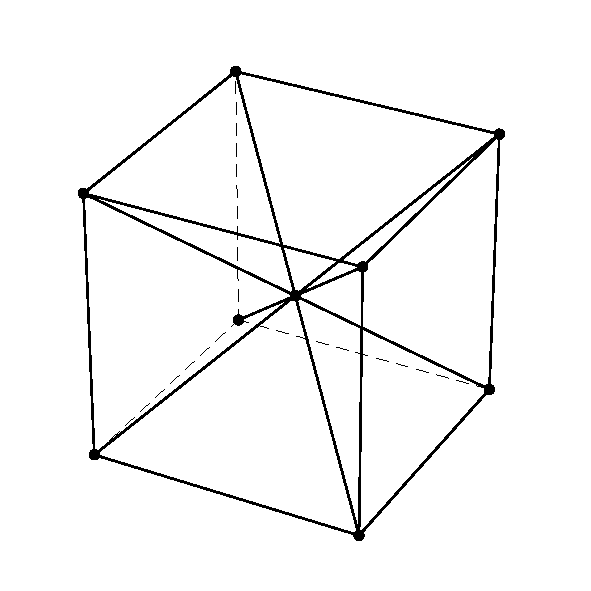
\includegraphics[scale=0.8]{fig/1-cube.pdf}
    \caption{Cube and its Diagonals}
    \label{fig:cube-diagonals}
\end{figure}

\begin{example}[Symmetry of the Cube]
    \label{ex:symmetry-of-cube}
    Let \(G\) be the symmetry group of the cube, and let \(X\) be the set of diagonals (between opposite vertices), as in \autoref{fig:cube-diagonals}. Then \(G \actson X\).

    Consider the associated  homomorphism \(\functiondomain{\phi}{G}{\Sym\pqty{X} \isomorphic S_4}\).
    
    We first show that \(\img \pqty{\phi} \isomorphic S_4\), and this can be shown by showing the transpositions lie in the image. This is trivial and left as an exercise.

    Now, consider the kernel of this map. There are two maps that keeps the diagonal unchanged: one is trivial (the identity), and one is which sends every vertex to its opposite. This means \(\ker \pqty{\phi} \isomorphic C_2\).

    Hence, we have
    \[
        \abs{G} = \abs{S_4} \cdot \abs{C_2} = 48
    \]
    by \autoref{thm:lagrange} (Lagrange's Theorem) and \autoref{thm:first-isomorphism-theorem-groups} (First Isomorphism Theorem for Groups).
\end{example}

\begin{example}[Cayley's Theorem]
    \label{ex:cayley-theorem}%
    For any group \(G\), we can write \(G\) act on (the underlying set) \(G\) by
    \[
        \function{\alpha}{G \times G}{G}{\pqty{g_1, g_2}}{g_1 g_2.}
    \]

    This induces a homomorphism \(\functiondomain{\phi}{G}{\Sym\pqty{G}}\). The kernel is
    \[
        \ker\pqty{\phi} = \set{g \in G}{g \cdot g_1 = g_1 \text{ for all }g_1 \in G} = \Bqty{e}.
    \]

    So we have \(\phi\) is injective, and hence \(G\) is some subgroup of \(\Sym\pqty{G}\) by \autoref{thm:first-isomorphism-theorem-groups} (First Isomorphism Theorem for Groups).

    This tells us that the symmetric group is \emph{very} complicated!
\end{example}

\begin{example}[Left-Multiplication on Cosets and its Kernel]
    \label{ex:left-multiplation-cosets}%
    Let \(H \subgroup G\) and \(X = \flatfrac{G}{H}\). Let \(G \actson H\) by
    \[
        \function{\alpha}{G \times \flatfrac{G}{H}}{\flatfrac{G}{H}}{\pqty{g, g_1 H}}{\pqty{g \cdot g_1} H}.
    \]

    We get the corresponding homomorphism \(\functiondomain{\phi}{G}\Sym\pqty{X}\). Trivially, we have \(\ker\pqty{\phi} \subseteq H\).

    But we have more to this. If \(g \in \ker \pqty{\phi}\), then
    \[
        g \cdot g_1 H = g_1 H
    \]
    for \emph{all} \(g_1 \in G\). Therefore,
    \[
        g_1 \inverse g g_1 \in H,
    \]
    so
    \[
        \ker\pqty{\phi} \subseteq \bigcap_{g_1 \in G} g_1 H g_1 \inverse.
    \]

    This argument is however, indeed, reversible: if
    \[
        g \in \bigcap_{g_1 \in G} g_1 H g_1 \inverse,
    \]
    then for each \(g_1 \in G\), we have
    \[
        g_1 \inverse g g_1 \in H,
    \]
    which means
    \[
        g g_1 H = g_1 H
    \]
    which means \(g \in \ker\pqty{\phi}\).

    In other words, we have
    \[
        \ker\pqty{\phi} = \bigcap_{g_1 \in G} g_1 H g_1 \inverse.
    \]

    In the special case where \(H \normalsub G\), then \(\ker\pqty{\phi} = H\). But in the general case, the right-hand side is an intersection of subgroups, which induce a normal subgroup!
\end{example}

\begin{theorem}[Normal Subgroup in Subgroup]
    \label{thm:normal-subgroup-contained-in-subgroup}%
    Let \(G\) be finite and \(H \subgroup G\) of index \(n\). Then there exists a normal subgroup \(K \normalsub G\) which also satisfies \(K \subgroup H\), such that \(\flatfrac{G}{K}\) is isomorphic to  a subgroup of \(S_n\). Thus, \(\abs{\flatfrac{G}{K}}\) divides \(n!\) and \(\abs{\flatfrac{G}{K}} \geq n\).
\end{theorem}

\begin{proof}
    Consider \(\functiondomain{\phi}{G}{\Sym\pqty{\flatfrac{G}{H}}}\) induced by the action considered in \autoref{ex:left-multiplation-cosets}. The kernel is normal in \(G\), and we let \(K = \ker \pqty{\phi}\). We have already shown it is contained in \(H\).

    By \autoref{thm:first-isomorphism-theorem-groups} (First Isomorphism Theorem for Groups), we have
    \[
        \flatfrac{G}{K} \isomorphic \img \pqty{\phi} \subgroup \Sym\pqty{\flatfrac{G}{H}} \isomorphic S_n.
    \]

    \autoref{thm:lagrange} (Lagrange's Theorem) gives \(\abs{\flatfrac{G}{H}} \divides n!\), and \(K \subgroup H\), so \(\abs{\flatfrac{G}{K}} \geq \abs{\flatfrac{G}{H}} = n\).
\end{proof}

\begin{corollary}[Non-Abelian Simple Groups]
    \label{cor:non-abelian-simple-group}%
    Let \(G\) be a non-abelian simple group. Let \(H \subgroup G\) be a proper subgroup with index \(n > 1\). Then \(G\) is isomorphic to a subgroup of \(A_n\), where \(n \geq 5\).
\end{corollary}

\begin{proof}
    We consider the same action \(G \actson \flatfrac{G}{X}\) by left-multiplication, and the homomorphism induced
    \[
        \functiondomain{\phi}{G}{\Sym\pqty{\flatfrac{G}{H}} \isomorphic S_n}.
    \]

    We look at its kernel. Since \(\ker \phi \normalsub G\), and \(G\) is simple, there are only two possibilities: \(\ker \phi = \Bqty{e}\) or \(\ker \phi = G\).

    But since \(\ker \phi \subgroup H\), and \(H\) is a proper subgroup, we have \(\ker \phi = \Bqty{e}\), so the homomorphism is injective, and by \autoref{thm:first-isomorphism-theorem-groups} (First Isomorphism Theorem for Groups),
    \[
        G \isomorphic \img \pqty{\phi} \subgroup \Sym\pqty{\flatfrac{G}{H}} \isomorphic S_n.
    \]

    For simplicity of notation, identify \(G\) with \(\img \pqty{\phi}\) and \(\Sym\pqty{\flatfrac{G}{H}}\) with \(S_n\). We know that
    \[
        G \subgroup S_n
    \]
    and we in fact want \(G \subgroup A_n\), i.e., \(G \cap A_n = G\).

    Since \(A_n \normalsub S_n\), we must have \(A_n \cap G \normalsub G\). This is by \autoref{thm:second-isomorphism-theorem-groups} (Second Isomorphism Theorem for Groups). But \(G\) is simple, so \(G \cap A_n = \Bqty{e}\), or \(G \cap A_n = G\).

    We need to rule out the case where \(G\) intersects \(A_n\) trivially. To see this, again, using \autoref{thm:second-isomorphism-theorem-groups} (Second Isomorphism Theorem for Groups), if \(G \cap A_n = \Bqty{e}\), we see that
    \[
        G \isomorphic \flatfrac{G}{G \cap A_n} \isomorphic \flatfrac{G A_n}{A_n} \leq \flatfrac{S_n}{A_n} \isomorphic C_2,
    \]
    but this is stupid since \(G\) is non-abelian.

    We last directly verify that \(S_1\) and \(S_2\) are abelian, and \(S_3\) and \(S_4\) has no non-abelian simple subgroup.
\end{proof}

\begin{definition}[Orbits, Stabalisers]
    \label{def:orbits-stablisers}%
    Let \(G \actson X\) be a group action. Let \(x \in X\).
    
    \begin{itemize}
        \item The \emph{orbit} of \(x\), denoted as \(G x\), is defined to be
        \[
            G x = \set{gx}{g \in G} \subseteq x.
        \]
        \item The \emph{stabiliser}  of \(x\), denoted as \(G_x\),is defined to be
        \[
            \set{g \in G}{gx = x} \subgroup G.
        \]
    \end{itemize}
\end{definition}

\begin{theorem}[Orbit--Stabiliser]
    \label{thm:orbit-stabiliser}%
    For \(G \actson X\) and \(x \in X\), the map \(\phi\) given as follows, is a bijection.

    \[
        \function{\phi}{Gx}{\flatfrac{G}{G_x}}{gx}{g G_x}
    \]
    
    In particular, if \(G\) is finite, we have
    \[
        \abs{G} = \abs{Gx} \cdot \abs{G_x}.
    \]
\end{theorem}
\section{Conjugacy, Centralisers and Normalisers}

A group \(G\) can act on itself by conjugation as
\[
    \function{\ast}{G \times G}{G}{\pqty{g, h}}{g h g\inverse}.
\]

\begin{lemma}[Conjugation by Element gives Homomorphism from the Group to Itself]
    \label{lem:conjugation-element-homomorphism-self}%
    If we fix \(g \in G\), the permutation
    \[
        \function{\pi}{G}{G}{h}{ghg\inverse}
    \]
    gives a homomorphism from \(G\) to itself.
\end{lemma}

\begin{definition}[Automorphism, Automorphism Group]
    \label{def:automorphism}%
    Let \(G\) be a group. A permutation \(G \to G\) is an \emph{automorphism} if it is also a homomorphism.

    The set of all automorphisms of \(G\) form a group, namely the \emph{automorphism group}, denoted as
    \[
        \Aut\pqty{G} = \set{\functiondomain{f}{G}{G}}{f \text{ is an automorphism}} \subgroup \Sym\pqty{G}.
    \]
\end{definition}

\begin{example*}
    Let \(G = \RR^2\) be under addition. Then \(\Aut\pqty{G} \supgroup \GL_2\pqty{\RR}\).
\end{example*}

\begin{notation}
    The automorphisms given by conjugation action are called \emph{inner automorphisms}, denoted as \(\Inn\pqty{G}\). This is a normal subgroup of \(\Aut\pqty{G}\), and the quotient is the \emph{outer automorphism group}, denoted as \(\Out\pqty{G}\).
\end{notation}

\begin{definition}[Conjugation Class, Centraliser, Centre]
    \label{def:ccl-centraliser-centre}%
    Fix \(g \in G\). The \emph{conjugacy class} of \(g\) is the orbit under conjugation action, given by
    \[
        \ccl_G\pqty{g} = \set{hgh\inverse}{h \in G}.
    \]

    The \emph{centraliser} of \(g \in G\) is the stabiliser under conjugation action, given by
    \[
        C_G\pqty{g} = \set{h \in G}{h g h\inverse = g}.
    \]

    The \emph{centre} of \(G\) is the kernel of conjugation action, given by
    \[
        Z\pqty{G} = \set{z \in G}{\forall g \in G: zg = gz}.
    \]
\end{definition}

\begin{proposition}[Size of Conjugacy Class]
    \label{prop:size-conjugacy-class}%
    Let \(G\) be a finite group. Then for all \(x \in G\), we have
    \[
        \abs{\ccl\pqty{x}} = \abs{G : C_G\pqty{x}} = \frac{\abs{G}}{\abs{C_G\pqty{x}}}.
    \]
\end{proposition}

\begin{proof}
    Apply \autoref{thm:orbit-stabiliser} (Orbit--Stabiliser Theorem).
\end{proof}

\begin{definition}[Normaliser]
    \label{def:normaliser}%
    Let \(H \subgroup G\). The \emph{normaliser} of \(H \in G\) is
    \[
        N_G \pqty{H} = \set{g \in G}{gHg\inverse = H}.
    \]
\end{definition}

Observe that \(H \normalsub N_G\pqty{H}\), and in fact by definition, \(N_G\pqty{H}\) is the \emph{largest} subgroup of \(G\), inside which \(H\) is normal.
\section{Simplicity of the Alternating Groups}

Recall that a conjugacy class in \(S_n\) consists of the set of all elements of a fixed cycle type.

\begin{example}
    For example, all the \(\para{2, 3}\)-cycles in \(S_5\) form a conjugacy class.
\end{example}

\begin{theorem}[Simplicity of \(A_n\) for \(n \geq 5\)]
    \label{thm:an-simple}%
    Let \(n \geq 5\). Then \(A_n\) is simple.
\end{theorem}

\begin{proof}
    There are three steps of the proof:
    \begin{enumerate}
        \item \(A_n\) is generated by \(3\)-cycles;
        \item Any \(H \normalsub A_n\) that contains a \(3\)-cycle contains all of them;
        \item Any non-trivial \(H \normalsub A_n\) does contain a \(3\)-cycle.
    \end{enumerate}

    It should be clear that the three statements combined gives the desired statement. Note in particular that the second statement is not trivial -- since we are working in \(A_n\), not \(S_n\).

    \begin{proof}[of 1]
        Any \(g \in A_n\) is a product of evenly-many transpositions. We consider pairs of transpositions, then this gives three possibilities:
        \begin{itemize}
            \item \(\perm{ab} \perm{ab} = e\).
            \item \(\perm{ab} \perm{bc} = \perm{abc}\) is a \(3\)-cycle.
            \item \(\perm{ab} \perm{cd} = \perm{acb} \perm{acd}\) is a product of \(3\)-cycles.
        \end{itemize}
    \end{proof}

    \begin{proof}[of 2]
        Any two \(3\)-cycles are conjugate when viewed in \(S_n\). Let \(\delta, \delta'\) be \(3\)-cycles, then we may write
        \[
            \delta' = \sigma \delta \sigma\inverse
        \]
        for \(\sigma \in S_n\). But observe that \(n \geq 5\), so there is some transposition \(\tau \in S_n\) disjoint from \(\delta\), which means it commutes with \(\delta\). Therefore,
        \[
            \delta' = \para{\sigma \tau} \delta \para{\tau\inverse \sigma\inverse} = \para{\sigma \tau} \delta \para{\sigma \tau}\inverse
        \]
        and hence \(\sigma \tau \in A_n\), showing \(\delta\) and \(\delta'\)are conjugate in \(A_n\).
    \end{proof}
\end{proof}
\section{Finite \(p\)-Groups}

Let \(p\) be a prime. Groups of order \(p^n\) for \(n \geq 1\) are often called \(p\)-groups, which have certain properties that are interesting.

\begin{theorem}[\(p\)-Groups have Non-Trivial Centres]
    \label{thm:p-groups-non-trivial-centre}%
    Let \(G\) be a \(p\)-group. Then the centre of \(G\) is non-trivial.
\end{theorem}

\begin{proof}
    Let \(G \actson G\) by conjugation. Then the centre \(Z\pqty{G}\) is the set of all size-\(1\) orbits. The orbits in this case partition \(G\), so we can write
    \[
        \abs{G} = p^n = \abs{Z\pqty{G}} + \sum_{\abs{\ccl\pqty{g}} > 1} \abs{\ccl\pqty{g}}
    \]

    We know every conjugacy class has sizes that divide \(p^n\). If they are bigger than \(1\), then \(p\) divides the size. Therefore, \(p \divides \abs{G}\) and the sum of the conjugacy class sizes larger than \(1\).

    Therefore, \(p \divides Z\pqty{G}\), giving \(\abs{Z\pqty{G}} \geq p\).
\end{proof}

\begin{theorem}[Groups of Order \(p^2\) is Abelian]
    \label{thm:order-p2-abelian}%
    A group of size \(p^2\) is always abelian.
\end{theorem}

\begin{lemma}[Quotient by Centre being Cyclic implies Abelian]
    \label{lem:quotient-by-centre-cyclic-abelian}%
    If \(\flatfrac{G}{Z\pqty{G}}\) is cyclic, then \(G\) is abelian.
\end{lemma}

\begin{proof}
    That \(\flatfrac{G}{Z\pqty{G}}\) is cyclic implies that there is some coset \(x Z \pqty{G} \in \flatfrac{G}{Z\pqty{G}}\) that generates the whole quotient. In other words, every coset has the form \(x^m Z\pqty{G}\), for some \(m \geq 0\).

    Since every \(g \in G\) can be written as some \(g = x^m z\) for some \(m \geq 0, z \in Z\pqty{G}\).

    Let \(g = x^m z\) and \(h = x^n z'\), then
    \[
        g h = x^m z x^n z' = x^{m + n} z z' = x^{n + m} z' z = x^n z' x^m z = h g
    \]
    indeed. (Every element is a power of a fixed element times something that commutes with every element.)
\end{proof}

\begin{proof}[\proofname\ of \autoref{thm:order-p2-abelian}]
    Using \autoref{thm:p-groups-non-trivial-centre}, we have \(Z\pqty{G}\) is either order \(p\) or \(p^2\), and in the latter case we are done.

    But if \(\abs{Z\pqty{G}} = p\), then \(\flatfrac{G}{Z\pqty{G}}\) is cyclic, so \(G\) is abelian, contradicting with \(\abs{Z\pqty{G}} = p\).
    
    So \(\abs{Z\pqty{G}} = p^2\) and \(G\) is indeed abelian.
\end{proof}

\begin{theorem}[\(p\)-Groups have Subgoups of order Powers of \(p\)]
    \label{thm:p-group-subgoup-order-power-of-p}
    Let \(G\) be a \(p\)-group of size \(p^n\). Then \(G\) has a subgroup of size \(p^{k}\) for all \(0 \leq k \leq n\).
\end{theorem}

\begin{proof}
    We conduct induction on \(n\). For the \(n = 1\) case, this is trivially true, since \(G \isomorphic C_p\).

    If \(n > 1\), if \(k = 0\), take \(\Bqty{e}\), and so we are done.

    Otherwise, note that the centre \(Z\pqty{G}\) is non-trivial, and for \(x \in G\) where \(x \neq e\), we have \(\ord\pqty{x}\) is a power of \(p\). If we replace with a power of itself, we can assume it has order exactly \(p\). (Alternatively, \(p\) divides the order of \(Z\pqty{G}\) and apply Cauchy's Theorem.)

    Then, \(\angBrac{x}\) has order \(p\), and since \(x \in Z\pqty{G}\), we have \(\angBrac{x} \normalsub G\). This allows us to take the quotient \(\flatfrac{G}{\angBrac{x}}\). This is a group of size \(p^{n - 1}\), and by induction it contains some subgroup of size \(p^{k - 1}\), call it \(L \subgroup \flatfrac{G}{\angBrac{X}}\).

    But by the correspondence result (between the subgroups of \(G\) and subgroups of the quotient), we find some \(K \subgroup G\) containing \(\angBrac{x}\), such that \(\flatfrac{K}{\angBrac{x}} \isomorphic L\). This gives \(\abs{K} = p^k\) ad so we are done.
\end{proof}
\section{Finite Abelian Groups}

\begin{theorem}[Classification of Finite Abelian Groups]
    \label{thm:classification-finite-abelian-group}%
    Let \(G\) be a finite abelian group. Then \(G\) must be a product of cyclic groups. More precisely, there exist positive integers \(d_1, \ldots, d_r\), such that
    \[
        G \isomorphic C_{d_1} \times \cdots \times C_{d_r}.
    \]

    Moreover, we can choose the \(d_i\) such that \(d_{i + 1} \divides d_i\), in which case the expression is unique.
\end{theorem}

The proof will not be until the end of the course, where we prove the Structure Theorem for Finitely-Generated Modules over a PID (Principle Ideal Domain) -- the PID Structure Theorem -- which would imply also, the existence of the Smith normal form and the Jordan normal form. (P.S. \href{https://pumac.princeton.edu/archives#2022}{PUMaC 2022* Power Round} has a good introduction to this -- \href{https://static1.squarespace.com/static/570450471d07c094a39efaed/t/642304302502a43377dedfed/1680016432869/PUMaC2023PowerRoundMarch28Update.pdf}{the questions are linked})

\begin{example}[Abelian Groups of Order \(8\)]
    The only abelian groups of order \(8\) are exactly \(C_8\), \(C_4 \times C_2\), and \(C_2 \times C_2 \times C_2\).
\end{example}

\begin{lemma}[Chinese Remainder Theorem]
    \label{lem:chinese-remainder-theorem}
    If \(n, m\) are coprime, then \(C_n \times C_m \isomorphic C_{nm}\).
\end{lemma}

\begin{proof}
    It suffices to find an order \(nm\) element in \(C_n \times C_m\). If \(g \in C_n\) is order \(n\) and \(h \in C_m\) is order \(m\), then consider \(\para{g, h} \in C_n \times C_m\).

    Suppose it has order \(k\). Then \(\para{g, h}^k = \para{g^k, h^k} = \para{e, e}\). Coordinate-wise, we may conclude that \(n \divides k\) and \(m \divides k\). But \(\gcd\para{m, n} = 1\), so \(nm \divides k\).
    
    But \(k \divides mn\) as well by \autoref{thm:lagrange} (Lagrange's Theorem), so \(k = mn\).
\end{proof}

\begin{corollary}[Finite Abelian Groups as Prime Powers]
    \label{cor:finite-abelian-groups-prime-powers}
    If \(G\) is a finite, abelian group, then we have
    \[
        G \isomorphic C_{l_1} \times C_{l_2} \times \cdots \times C_{l_n}
    \]
    where each \(l_i\) is a prime power, not necessarily of distinct primes.
\end{corollary}

\begin{proof}
    Combine \autoref{lem:chinese-remainder-theorem} and \autoref{thm:classification-finite-abelian-group}.
\end{proof}

This is another form of the factorisation of finite abelian groups into cyclic groups. For example, in \autoref{thm:classification-finite-abelian-group}, \(C_6 \isomorphic C_6\), but here, \(C_6 \isomorphic C_2 \times C_3\) is the alternative factorisation.
\section{Sylow Theorem}

Let \(G\) be a finite group of size \(p^{a} m\) where \(p \notdivides m\), which means we collected all the prime factors \(p\) in the first part of the product. A \emph{Sylow \(p\)-Subgroup} of \(G\) is a subgroup of order \(p^a\).

\begin{theorem}[Sylow Theorems]
    \label{thm:sylow}%
    Let \(G\) be a finite group, and let \(p\) be a prime, with \(p \divides \abs{G}\).

    \begin{enumerate}
        \item The set \(\Syl_p\para{G} = \set{P \leq G}{P \text{ is a Sylow } p\text{-subgroup}}\) is non-empty.
        \item Any \(H, H' \in \Syl_p \para{G}\) are conjugate, i.e., there is some \(g\) such that \(H' = g H g\inverse\).
        \item If \(n_p = \abs{\Syl_p \para{G}}\), then \(n_p \equiv 1 \pmod{p}\), and hence \(n_p\) divides \(\abs{G}\), so \(m\).
    \end{enumerate}
\end{theorem}

The first part of \autoref{thm:sylow} (Sylow Theorem) itself is already very interesting -- since it is not easy to specify that we have a subgroup is of a particular size. The second is also non-trivial, since there could be subgroups with different structures, or with the same structure but not conjugate. Nevertheless, we will build up the necessary foundations to a proof.

\begin{lemma}[Unique Sylow \(p\)-Subgroup implies Normality]
    If \(\Syl_p\para{G} = \brce{P}\) has size \(1\), then \(P\) is normal.
\end{lemma}

\begin{proof}
    For any \(g \in G\), \(g P g\inverse\) is isomorphic to \(P\) as a subgroup, so we have \(g P g\inverse \in \Syl_p\para{G}\). It follows that \(P = g P g\inverse\), and this finishes a proof.
\end{proof}

Another consequence of Sylow's theorem is as follows.

\begin{corollary}[Number of Sylow \(p\)-Subgroups and Size of \(G\)]
    \label{cor:np-and-g}%
    Let \(G\) be a non-abelian simple group and let \(p \divides \abs{G}\). Then \(\abs{G}\) divides \(\frac{n_p!}{2}\), and \(n_p \geq 5\).
\end{corollary}

\begin{proof}
    The conjugation action of \(G\) on \(\Syl_p\para{G}\) gives a homomorphism
    \[
        \functiondomain{\phi}{G}{\Sym\para{\Syl_p\para{G}} \isomorphic S_{n_p}}.
    \]

    By simplicity of \(G\), since \(\ker \phi \normalsub G\), we therefore have \(\ker \phi = \brce{e}\) or \(\ker \phi = G\).

    If \(\ker \phi = G\), this means the conjugation action is trivial, so \(g P g\inverse = P\) for all \(g \in G\), then \(P\) is normal. Since \(P \neq \brce{e}\), we must have \(G = P\). But this is impossible, because \autoref{thm:p-groups-non-trivial-centre} (\(p\)-groups have Non-Trivial Centres) gives a normal subgroup \(Z\para{P} \normalsub P\).

    Therefore, \(\ker \phi = \brce{e}\), so \(\phi\) is injective, and hence \(G\) must be isomorphic a subgroup of \(S_{n_p}\). We want to make sure it lies in \(A_{n_p}\). We consider the composition

    \[
        G \overset{\phi}{\longrightarrow} S_{n_p} \overset{\sign}{\longrightarrow} \brce{\pm 1}.
    \]

    If the composition is surjective, then \(\ker \para{\sign \circ \phi}\) is an index \(2\) subgroup of \(G\). But \(G\) is simple, so this is impossible, unless \(G \isomorphic C_2\) but this is abelian. (Alternatively, since this composition cannot be injective and since \(G\) is simple, we have \(\ker \para{\sign \circ \phi} = G\), so this map is trivial.)

    Therefore, \(\img \para{\phi} \subgroup A_{n_p}\) and we have \(\frac{n_ p!}{2}\), so we can calculate by Lagrange.

    Now we may verify directly that \(A_1, A_2, \ldots, A_4\) are not simple directly.
\end{proof}

A nice application of the numerology provided by \autoref{thm:sylow} (Sylow's Theorems) is explored below.

\begin{example*}[Counting Subgroups of Simple Group]
    Suppose \(G\) has size \(11 \times 12 = 132\). If \(g\) is simple, then none of the \(n_p\)s are equal to \(1\).

    By \autoref{thm:sylow} (Sylow's Third Theorem), we have \(n_{11} \equiv 1 \pmod{11}\) but also \(n_{11} \divides 12\), so \(n_{11} = 12\), so there are \(12\) Sylow \(11\)-subgroups.

    Similarly, we know that \(n_3 \equiv 1 \pmod{3}\) and \(n_3 \divides 44\). So by simplicity, \(n_3 = 4\) or \(22\).

    By \autoref{cor:np-and-g}, we have \(n_3 = 22\) since \(n_3 \geq 5\).

    Any two Sylow \(11\)-Subgroups intersect trivially at \(\brce{e}\), which gives already \(120\) elements. Similarly, any two Sylow \(3\)-Subgroups contribute another \(44\) elements. But we only have a total of \(132\) elements, which is impossible.
\end{example*}

Now we prove Sylow's theorems.

\begin{proof}[of Sylow's First Theorem, Part of \autoref{thm:sylow}]
    We produce a Sylow \(p\)-Subgroup as a stabiliser of an orbit in an appropriate action.
    
    Let \(\abs{G} = n = p^a m\) with \(p \notdivides m\). Define the collection of \textbf{subsets} (not subgroups!)
    \[
        \Omega = \set{X \subseteq G}{\abs{X} = p^a} \subseteq \powerset\para{G}.
    \]

    Let \(G\) act on \(\Omega\) by left-multiplication element-wise, i.e.,
    \[
        g \ast \brce{g_1, g_2, \ldots, g_{p^a}} = \brce{g g_1, \ldots, g g_{p^a}}.
    \]

    We want to have an orbit of size \(m\), so its stabiliser would have size \(p^a\).

    We first claim that \(\abs{\Omega} = \binom{n}{p^a} \equiv m \nequiv 0 \pmod{p}\). This part is elementary algebra.

    The second claim is that, if \(U \in \Omega\), and \(H \subgroup G\) stabilises \(U\), then \(\abs{H} \divides \abs{U}\).
    
    Since \(H\) stabilises \(U\), this means \(hU = U\) for all \(h \in H\). In other words, for each \(u \in U\), the coset \(Hu\) is contained in \(U\). Every \(u \in U\) lies in some coset of \(H\), and since cosets are disjoint with same size, they therefore partition \(U\), we get \(\abs{H} \divides \abs{U}\).

    Now, we know that \(\abs{\Omega} \nequiv 0 \pmod{p}\), and by partitioning of orbits \(O_i\), we have
    \[
        \abs{\Omega} = \abs{O_1} + \abs{O_2} + \cdots + \abs{O_r}.
    \]

    Since \(p \notdivides \abs{\Omega}\), there exists an orbit, say \(\Theta\), whose size is not a multiple of \(p\).

    Let \(X \in \Theta\). By \autoref{thm:orbit-stabiliser}, we have
    \[
        \abs{G} = \abs{\Theta} \cdot \abs{\Stab\para{X}},
    \]
    so \(p^a m = \abs{\Theta} \cdot \abs{\Stab\para{X}}\).

    Since no factors of \(p\) is in \(\abs{\Theta}\), they must be wholly contained in \(\abs{\Stab\para{X}}\), i.e., \(p^a \divides \abs{\Stab\para{X}}\). But by definition of \(\Omega\), we have \(\abs{X} = p^a\), and by the second claim, \(\abs{\Stab\para{X}} \divides p^a\).

    Therefore, \(\abs{\Stab\para{X}} = p^a\) is a Sylow \(p\)-Subgroup which finishes our proof.
\end{proof}
\section{Basic Concepts of Rings}

Good examples of rings to keep in mind are \(\ZZ, \ZZ / n, \RR \brac{x}\).

\begin{definition}[Ring]
    \label{def:ring}%
    A \emph{ring} is a quintuple \(\para{R, +, \cdot, 0_R, 1_R}\) where \(R\) is a set, \(0_R, 1_R \in R\), and
    \begin{align*}
        \functiondomain{+&}{R \times R}{R} && \text{``addition''} \\
        \functiondomain{\cdot&}{R \times R}{R}, && \text{``multiplication''}
    \end{align*}
    such that
    \begin{itemize}
        \item \(\para{R, +, 0_R}\) is an abelian group;
        \item the operation \(\cdot\) is associative: for all \(a, b, c \in R\), \(a \cdot \para{b \cdot c} = \para{a \cdot b} \cdot c\);
        \item \(1_R\) is a multiplicative identity for \(R\): for all \(a \in R\), \(1_R \cdot a = a \cdot 1_R = a\);
        \item multiplication is distributive over addition: for all \(r_1, r_2, r_3 \in R\), \(r_1 \cdot \para{r_2 + r_3} = r_1 \cdot r_2 + r_1 \cdot r_3\), and \(\para{r_1 + r_2} \cdot r_3 = r_1 \cdot r_3 + r_2 \cdot r_3\).
    \end{itemize}
\end{definition}

\begin{notation}
    We will denote this as ``\(R\) is a ring''. The symbol \(-r\) will mean the additive inverse of \(r\), and note \(r - s = r + \para{-s}\).
\end{notation}

\begin{remark}
    In this course, all rings are assumed to \emph{commutative}, that \(r_1 \cdot r_2 = r_2 \cdot r_1\) for all \(r_1, r_2 \in R\).
\end{remark}

\begin{definition}[Subring]
    \label{def:subring}%
    A \emph{subring} of a ring \(R\) is a subset \(S \subseteq R\), such that \(0_R, 1_R \in S\), and if \(s, s' \in S\), then \(s + s', s \cdot s'\) also lie in \(S\), and \(\para{S, +, \cdot, 0_R, 1_R}\) is a ring.

    We note this as \(S \subring R\).
\end{definition}

\begin{example}[Examples of Rings]
    \label{ex:rings}%
    We have (the familiar number sets)
    \[
        \ZZ \subring \QQ \subring \RR \subring \CC
    \]
    are all rings.

    The \emph{Gaussian Integers} is
    \[
        \ZZ \brac{i} = \set{a + ib}{a, b \in \ZZ} \subring \CC.
    \]

    Similarly,
    \[
        \QQ \brac{\sqrt{2}} = \set{a + b \sqrt{2}}{a, b \in \QQ} \subring \RR.
    \]

    Less familiarly,
    \[
        \CC \ang{\epsilon} = \set{a + b\epsilon}{a, b \in \CC}
    \]
    with operations
    \[
        \para{a + b\epsilon} + \para{c + d\epsilon} = \para{a + c} + \para{b + d}\epsilon
    \]
    and
    \[
        \para{a + b\epsilon} \cdot \para{c + d\epsilon} = ac + \para{ad + bc} \epsilon,
    \]
    with
    \[
        0 = 0 + 0 \cdot \epsilon, 1 = 1 + 0 \cdot \epsilon.
    \]

    This is the ring of \emph{dual numbers}. In particular, \(\epsilon^2 = 0\) even though \(\epsilon \neq 0\).
\end{example}

\begin{definition}[Unit]
    \label{def:unit}%
    An element \(u \in R\) is a \emph{unit} if there exists \(v \in R\), such that \(uv = 1\).
\end{definition}

\begin{remark}
    Note that \(2 \in \ZZ \subring \QQ\), and \(2\) is a unit in \(\QQ\), but \textbf{not in \(\ZZ\)}. A unit in a ring is not necessarily a unit in a subring: \textbf{subrings do not preserve units}.
\end{remark}

\begin{definition}[Field]
    \label{def:field}%
    A ring \(R\) is a \emph{field} if every non-zero element is a unit.
\end{definition}

Note that the product of units must be a unit, although their sum might not be. The units form a subgroup under multiplication.
\section{Homomorphisms, Ideals and Quotients}

\begin{definition}[Ring Homomorphism]
    \label{def:ring-homomorphism}%
    Let \(R\) and \(S\) be rings. A function \(\functiondomain{f}{R}{S}\) is a \emph{ring homomorphism} if
    \begin{enumerate}
        \item \(f\pqty{r_1 + r_2} = f\pqty{r_1} + f\pqty{r_2}\);
        \item \(f\pqty{0} = 0\);
        \item \(f\pqty{r_1 r_2} = f\pqty{r_1} f\pqty{r_2}\);
        \item \(f\pqty{1} = 1\).
    \end{enumerate}
\end{definition}

\begin{remark}
    Point 4 is \textbf{not implied by} Point 3 (unlike Point 2 is implied by Point 1) since addition and multiplication are not symmetric -- addition gives a group structure, but multiplication does not (we cannot invert multiplication).
\end{remark}

\begin{definition}[Ring Isomorphism, Kernel, Image]
    \label{def:ring-isomorphism-kernel-image}%
    If \(\functiondomain{f}{R}{S}\) is a bijective ring homomorphism, it is an \emph{isomorphism}.

    The \emph{kernel} and \emph{image} of \(f\) is the kernel and image of the corresponding group homomorphism (when the operation is restricting to addition), i.e.,
    \[
        \ker f = \set{r \in R}{f \pqty{r} = 0}
    \]
    and
    \[
        \img f = \set{s \in S}{\exists r \in R: s = f\pqty{r}}.
    \]
\end{definition}

\begin{remark}
    The inverse of a ring isomorphism is also a ring isomorphism.
\end{remark}

\begin{lemma}[Homomorphisms are Injective if and only if it has Trivial Kernel]
    \label{lem:homomorphisms-injective-trivial-kernel}%
    A ring homomorphism \(\functiondomain{f}{R}{S}\) is injective if and only if \(\ker f = \Bqty{0}\).
\end{lemma}

\begin{proof}
    This is implied from the statement on group homomorphisms.
\end{proof}

Recall a group homomorphism's kernel must be a \emph{normal subgroup} -- there is a very similar key notion in rings.

\begin{definition}[Ideal]
    \label{def:ideal}%
    A subset \(I \subseteq R\) is called an \emph{ideal}, written as \(I \idealsub R\), if
    \begin{enumerate}
        \item \(I\) is a subgroup of \(R\) under addition; and
        \item \emph{Absorbing Rule.} If \(a \in I\) and \(b \in R\), then \(ab \in I\).
    \end{enumerate}
\end{definition}

\begin{remark}
    An ideal is not a subring, since it not necessarily contains \(1 \in R\). Indeed, if \(1 \in I \idealsub R\), then \(R = I\).
\end{remark}

\begin{lemma}[Kernels are Ideals]
    \label{lem:kernel-are-ideal}%
    If \(\functiondomain{\phi}{R}{S}\) is a homomorphism, then \(\ker \phi \idealsub R\) is an ideal.
\end{lemma}

\begin{proof}
    Since \(\phi\) is a group homomorphism, \(\ker \phi\) is a subgroup under addition.

    If \(a \in \ker \phi\) and \(b \in R\), then
    \[
        \phi\pqty{ab} = \phi\pqty{a} \cdot \phi\pqty{b} = 0 \cdot \phi\pqty{b} = 0
    \]
    so \(ab \in \ker \phi\), which finishes the proof.
\end{proof}

\begin{remark}
    Let \(u \in R\) is a unit, and \(I \idealsub R\) is an ideal. If \(u \in I\), then \(I = R\). This is since \(1 = u v\) for \(u \in I\) and \(v \in R\), then \(1 \in I\).
\end{remark}

\begin{example}[Ideals of \(\ZZ\)]
    \label{ex:ideals-of-z}%
    Let \(\ZZ\) be the ring of integers. Then
    \[
        n \ZZ = \Bqty{\ldots, -2n, -n, 0, n, 2n, \ldots}
    \]
    is an ideal. In fact, every (non-zero) ideal of \(\ZZ\) has this form, for some \(n \in \ZZ\). This result follows from the subgroup structure of \(\ZZ\), but we reproduce the proof of follows to motivate an algebraic structure.

    Indeed, if \(I \neq \Bqty{0}\), let \(n \in \ZZ\) be the smallest positive element \(n\) that lies in \(I\). We claim \(I = n\ZZ\).

    By the Euclidean algorithm, \(m = q \cdot n + r\) for \(q \in \ZZ\) and \(0 \leq r < n\), but \(q \cdot n \in I\) by definition of an ideal, so \(r \in I\). If \(r \neq 0\), then this contradicts minimality. So \(r = 0\) and this finishes the proof.
\end{example}

But we may generalise this idea -- this only required the Euclidean algorithm -- and we may abstract this to algebraic structures where such an `Euclidean algorithm' exists.

\begin{definition}[Ideal Generated by a Set, Principal Ideal]
    \label{def:ideal-generated-principal}%
    Let \(A \subseteq R\) be a subset. The \emph{ideal generated by \(A\)} is given by
    \[
        \pqty{A} = \set{\sum_{a \in A} r_a a}{r_a \in R, r_a = 0 \text{ for all but finitely many }a}.
    \]

    An ideal \(I \idealsub X\) is called \emph{principal} if \(A = \pqty{r}\) for some \(r \in R\).
\end{definition}

For example, as we see above, all ideals of \(\ZZ\) are principal, since \(n\ZZ\) is generated by \(n\).

\begin{example}[Ideal Generated]
    \label{ex:ideal-generated}%
    The subset of \(\RR\bqty{x}\) given by
    \[
        \set{f\pqty{x} \in \RR\bqty{x}}{f\pqty{0} = 0},
    \]
    i.e. polynomials with zero constant term is an ideal. It is generated by the element \(x \in \RR\bqty{x}\).
\end{example}

\begin{definition}[Quotient Ring]
    \label{def:quotient-ring}%
    Let \(I \idealsub R\). The \emph{quotient ring} is the set of cosets of \(I \in R\), taking the form \(\pqty{r + I}\) with \(0\) given by \(0_R + I\) and \(1\) given by \(1_R + I\), and operations
    \begin{align*}
        \pqty{r_1 + I} + \pqty{r_2 + I} &= \pqty{r_1 + r_2} + I, \\
        \pqty{r_1 + I} \cdot \pqty{r_2 + I} &= \pqty{r_1 \cdot r_2} + I.
    \end{align*}
\end{definition}

\begin{proposition}[Quotient Ring is a Ring]
    \label{prop:quotient-ring-ring}%
    The quotient ring \(\flatfrac{R}{I}\) is a ring, and the function
    \[
        \function{q_I}{R}{\flatfrac{R}{I}}{r}{r + I}
    \]
    is a ring homomorphism.
\end{proposition}

\begin{proof}
    Obviously, \(q_I\) is a well-defined group homomorphism and addition is well-defined. We verify that multiplication is well-defined (since it would suggest some motivation into why an ideal is defined in this particular way). Let
    \[
        r_1 + I = r_1' + I \qand r_2 + I = r_2' + I.
    \]

    Then \(r_1 - r_1' \in I\), say \(r_1 - r_1' = a_1\), and similarly let \(r_2 - r_2' = a_2 \in I\).

    Then
    \[
        r_1' r_2' = \pqty{r_1 + a_1} \pqty{r_2 + a_2} = r_1 r_2 + r_1 a_2 + r_2 a_1 + a_1 a_2.
    \]

    But \(r_1 a_2, r_2 a_1, a_1 a_2 \in I\) by absorption property. Therefore, we can conclude that
    \[
        r_1 r_2 + I = r_1' r_2' + I,
    \]
    so multiplication is indeed well-defined. The rest is straightforward.
\end{proof}

\begin{example}[Examples of Quotients]
    \label{ex:quotients}%
    \begin{itemize}
        \item We have ideals \(n \ZZ \idealsub \ZZ\). The quotient ring consists of the cosets
        \[
            \flatfrac{\ZZ}{n \ZZ} = \set{m + n \ZZ}{m \in \ZZ},
        \]
        and therefore we get \(0 + n \ZZ, 1 + n \ZZ, \ldots, \pqty{n - 1} + n\ZZ\). This ring structure takes the structure of arithmetic modulo \(n\).

        \item We take \(\pqty{x} \idealsub \CC\bqty{x}\). The elements of the quotient \(\flatfrac{\CC\bqty{x}}{\pqty{x}}\) can be represented by elements of the form
        \[
            \pqty{a_0 + a_1 x + \cdots + a_n x^n} + \pqty{x}.
        \]

        But the terms \(a_1 x, a_2 x^2, \ldots, a_n x^n \in \pqty{x}\), so this coset is equal to \(a_0 + \pqty{x}\). The representation is unique, so in fact
        \[
            \flatfrac{\CC \bqty{x}}{\pqty{x}} \isomorphic \CC.
        \]
    \end{itemize}
\end{example}

\begin{proposition}[Euclidean Algorithm for Polynomials]
    \label{prop:euclidean-algorithm-polynomials}%
    Let \(K\) be a field. If \(f, g \in K \bqty{x}\), then there exists \(r, q \in K \bqty{x}\), such that
    \[
        f = g \cdot q + r
    \]
    with \(\deg \pqty{r} < \deg \pqty{g}\).
\end{proposition}

\begin{proof}
    Let \(n = \deg \pqty{f}\), so \(f = \sum_{i = 0}^{n} a_i x^i\) where \(a_i \in K\) and \(a_n \neq 0\). Similarly, let \(g = \sum_{i = 0}^{m} b_i x_i\) where \(b_i \in K\) and \(b_m \neq 0\).

    If \(n < m\), set \(q = 0\) and \(r = f\) (purely remainder), and we are done.

    If \(n \geq m\), we proceed by induction on \(n\). Let \(f_1 = f - a_n b_m \inverse x^{n - m} g\). Note in particular, that \(b_m \inverse\) means we are using \(K\) is a \textbf{field}. So
    \[
        \deg \pqty{f_1} < n.
    \]

    If \(n = m\) then \(\deg \pqty{f_1} < n = m\), and hence
    \[
        f = \pqty{a_n b_m \inverse x^{n - m}} g + f_1.
    \]

    If \(n > m\), by induction, we can write \(f_1 = g q_1 + r_1\), where \(\deg \pqty{r_1} < \deg \pqty{g}\). Then,
    \[
        f = a_n b_m \inverse x^{n - m} g + q_1 g + r_1 = \pqty{a_n b_m \inverse x^{n - m} + q_1} g + r_1
    \]
    and we are done.
\end{proof}

A corollary of this is as follows: all ideals in \(K\bqty{x}\) for some field \(K\) are principal. This was shown in \autoref{ex:ideals-of-z}, and we may replace the Euclidean algorithm for \(\ZZ\) with \(K \bqty{x}\). However, note that \(\ZZ \bqty{x}\) and \(K \bqty{x, y}\) (where \(K\) is a field) \textbf{do not} have this property.

Similar to the isomorphism theorems we had in groups, we have them in rings as well.

\begin{theorem}[First Isomorphism Theorem for Rings]
    \label{thm:first-isomorphism-theorem-ring}%
    Let \(\functiondomain{\phi}{R}{S}\) be a ring homomorphism. Then the map
    \[
        \function{f}{\flatfrac{R}{\ker \phi}}{\img \phi \subring S}{r + \ker \phi}{\phi\pqty{r}}
    \]
    is a well-defined ring isomorphism.
\end{theorem}

\begin{proof}
    Bijectivity and additive property follows from \autoref{thm:first-isomorphism-theorem-groups} (First Isomorphism Theorem for Groups). It remains to show this is a ring homomorphism for multiplication. Indeed,
    \[
        f\pqty{\pqty{r + \ker \phi} \cdot \pqty{t + \ker \phi}} = f \pqty{rt + \ker \phi} = \phi \pqty{rt} = \phi\pqty{r} \phi\pqty{t} = f\pqty{r + \ker \phi} \cdot f\pqty{t + \ker \phi}.
    \]
\end{proof}

\begin{example}[Application of First Isomorphism Theorem]
    Consider the homomorphism
    \[
        \function{\phi}{\RR\bqty{x}}{\CC}{f\pqty{x}}{f\pqty{i}}.
    \]

    This map is surjective since \(\phi\pqty{a + bx} = a + bi\). 
    
    The kernel is exactly polynomials such that \(f\pqty{i} = 0\). But recall since this is a polynomial with real coefficients, if \(i\) is a root of \(f\), then so is \(\pqty{-i}\). So \(\pqty{x^2 + 1}\) divides \(f\pqty{x}\). Therefore, the kernel of \(\phi\) is \emph{exactly} \(\pqty{x^2 + 1} \idealsub \RR\bqty{x}\). Therefore, we have
    \[
        \CC \isomorphic \flatfrac{\RR\bqty{x}}{\pqty{x^2 + 1}}.
    \]
\end{example}

\begin{theorem}[Second Isomorphism Theorem for Rings]
    \label{thm:second-isomorphism-theorem-ring}%
    Let \(R \subring S\) and \(J \idealsub S\). Then \(R \cap J \idealsub R\), and \(\flatfrac{\pqty{R + J}}{J} = \set{r + J}{r \in R} \subring \flatfrac{S}{J}\). Furthermore,
    \[
        \flatfrac{R}{R \cap J} \isomorphic \flatfrac{\pqty{R + J}}{J}.
    \]
\end{theorem}

\begin{proof}
    Define a function
    \[
        \function{\phi}{R}{\flatfrac{S}{J}}{r}{r + J}.
    \]

    The kernel of this map is
    \[
        \ker \phi = \set{r \in R}{r + J = 0} = \set{r \in R}{r \in J} = R \cap J.
    \]

    We also have
    \[
        \img \phi = \set{r + J}{r \in R} = \flatfrac{\pqty{R + J}}{J}.
    \]

    By \autoref{thm:first-isomorphism-theorem-ring} (First Isomorphism Theorem for Rings), we have
    \[
        \flatfrac{R}{R \cap J} \isomorphic \flatfrac{\pqty{R + J}}{J}
    \]
    as rings.
\end{proof}

\begin{remark}
    Similar to rings, there is a correspondence for rings and ideals. Let \(I \idealsub R\) be an ideal. There is a bijection
    \[
        \function{f}{\Bqty{\text{subrings of }\flatfrac{R}{I}}}{\Bqty{\text{subrings of }R\text{ containing }I}}{L \subring \flatfrac{R}{I}}{\set{r \in R}{r + I \in L}}
    \]
    and the inverse is given by
    \[
        \function{f\inverse}{\Bqty{\text{subrings of }R\text{ containing }I}}{\Bqty{\text{subrings of }\flatfrac{R}{I}}}{I \idealsub S \subring R}{\flatfrac{S}{I} \subring \flatfrac{R}{I}.}
    \]
\end{remark}

\begin{theorem}[Third Isomorphism Theorem for Rings]
    \label{thm:third-isomorphism-theorem-ring}%
    Let \(I \idealsub R\) and \(J \idealsub R\), with \(I \subseteq J\). Then we have
    \[
        \flatfrac{J}{I} \idealsub \flatfrac{R}{I} \qand \flatfrac{\pqty{\flatfrac{R}{I}}}{\pqty{\flatfrac{J}{I}}} \isomorphic \flatfrac{R}{J}.
    \]
\end{theorem}

\begin{proof}
    Define the function
    \[
        \function{f}{\flatfrac{R}{I}}{\flatfrac{R}{J}}{r + I}{r + J.}
    \]

    It is well-defined by considering this as a group homomorphism.

    This is a ring homomorphism, with kernel
    \[
        \ker f = \set{r + I}{r + J = 0} = \flatfrac{J}{I}.
    \]

    Applying \autoref{thm:first-isomorphism-theorem-ring} (First Isomorphism Theorem for Rings) gives us the result, as desired.
\end{proof}

\begin{proposition}[Ring Homomorphism from \(\ZZ\), Characteristic of a Ring]
    \label{prop:ring-homomorphism-z-characteristic-of-ring}%
    Let \(R\) be any ring. Then there is a homomorphism
    \[
        \functiondomain{i}{\ZZ}{R}
    \]
    sending \(1\) to \(1_R\). For \(i\), we have
    \[
        \ker\pqty{i} = n \ZZ
    \]
    for some \(n \in \ZZ\), where \(\abs{n}\) is known as the \emph{characteristic} of \(R\).
\end{proposition}

Therefore, \(\ZZ\) is sometimes called the \emph{initial ring}. Furthermore, note that the zero ring does \textbf{not} have any homomorphisms to another ring (not a single one) -- this is different role from the trivial group back for group homomorphism.

\begin{example}[Characteristics of Common Rings]
    The infinite number rings \(\ZZ, \RR, \CC\) all have characteristic \(0\). The ring \(\flatfrac{\ZZ}{k\ZZ}\) has characteristic \(k\).
\end{example}
\section{Integral Domains, Fields of Fractions, Prime Ideals}

Notice that in the ring \(\flatfrac{\ZZ}{6}\), we have \(2 \cdot 3 = 0\) but \(2 \neq 0\) and \(3 \neq 0\).

\begin{definition}[Integral Domain, Zero Divisor]
    \label{def:integral-domain-zero-divisor}%
    A non-zero ring \(R\) is an \emph{integral domain}, if for all \(a, b \in R\), we have
    \[
        a b = 0 \implies a = 0 \qor b = 0.
    \]

    A \emph{zero divisor} if a non-zero \(a\), such that there exists \(b \neq 0\) if \(ab = 0\).
\end{definition}

For example, in \(\flatfrac{\ZZ}{6}\), we say both \(2\) and \(3\) are zero divisors.

\begin{examples}[Examples of Integral Domains]
    \label{ex:integral-domain}%
    \begin{itemize}
        \item Any field is an integral domain. Indeed, if \(a b = 0\) in a field, say \(b \neq 0\), then \(b\inverse\) exists, and
    \[
        a = a b b\inverse = a \cdot 0 = 0
    \]
    so \(a = 0\).
        \item Similarly, any subring of a field is also an integral domain. This is really how we should think of integral domains.
        \item The rings \(\ZZ\), \(\ZZ\bqty{i}\), \(\QQ\), \(\CC\), \(\RR\bqty{x}\) \(\ZZ\bqty{X}\) are integral domains.
        \item The rings \(\flatfrac{\ZZ}{6}\), \(\flatfrac{\ZZ}{\pqty{pq}}\), \(\flatfrac{\ZZ}{2} \times \flatfrac{\ZZ}{2}\), etc.
        \item In particular, direct products cannot be integral domains, since \(\pqty{0, 1}\) and \(\pqty{1, 0}\) product to \(0\).
    \end{itemize}
\end{examples}

\begin{lemma}[Finite Integral Domains are Finite Fields]
    \label{lem:finite-integral-domain-finate-field}%
    Let \(R\) be a finite integral domain. Then \(R\) is a field.
\end{lemma}

An example of this is \(\flatfrac{\ZZ}{p}\) for a prime \(p\).

\begin{proof}
    Let \(a \in R\) be non-zero, we want to prove it is a unit. Consider the multiplication function
    \[
        \function{\mu_a}{R}{R}{r}{ar.}
    \]

    This is a group homomorphism for the underlying group structure. Since \(R\) is an integral domain, by definition, we have
    \[
        \ker \pqty{\mu_a} = \Bqty{0}.
    \]

    So \(\mu_a\) is injective. Recall that \(R\) is finite, which means \(\mu_a\) is bijective.

    In particular, \(1 \in \img \pqty{\mu_a}\), so there is some \(b \in R\) with \(b \neq 0\), such that
    \[
        a \cdot b = 1
    \]
    so \(a\) is indeed a unit, finishing our proof.
\end{proof}

\begin{definition}[Field of Fractions]
    \label{def:field-of-fractions}%
    Let \(R\) be an integral domain. A \emph{field of fractions} of \(R\) is a field \(F\), such that
    \begin{enumerate}
        \item \(R \subring F\) is a subring, meaning there is an injective ring homomorphism from \(R\) to \(F\); and
        \item any \(x \in F\) can be written as \(a b \inverse\), for \(a, b \in R\), and \(b\inverse\) as the multiplicative inverse of \(b\) in \(F\).
    \end{enumerate}
\end{definition}

The first requirement is `sticking \(R\) into some field \(F\)', while the second requirement is `\(F\) is only contained of fractions in \(R\)'.

\begin{example*}[Field of Fractions of \(\ZZ\)]
    \label{ex:field-of-fractions-z}%
    The field \(\QQ\) is a field of fractions of \(\ZZ\).
\end{example*}

\begin{theorem}[Existence of Field of Fractions]
    \label{thm:existence-field-of-fractions}%
    Every integral domain \(R\) has a field of fractions.
\end{theorem}

Note \autoref{thm:existence-field-of-fractions} tells us that all integral rings are effectively subrings. The proof is inspired by the construction of \(\QQ\) by \(\ZZ\).

\begin{proof}
    Define a set
    \[
        S = \set{\pqty{a, b} \in R \times R}{b \neq 0}.
    \]

    We define a relation \(\sim\) over \(S\), being
    \[
        \pqty{a, b} \sim \pqty{c, d} \iff ad = bc,
    \]
    where here the multiplication is in \(R\).

    We want to show \(\sim\) is an equivalence relation. \emph{Symmetry} and \emph{reflective} are obvious. We conduct a non-trivial check on the \emph{transitivity}. Suppose that
    \[
        \pqty{a, b} \sim \pqty{c, d} \qand \pqty{c, d} \sim \pqty{e, f}.
    \]

    We have \(ad = bc\) and \(cf = de\). Multiplying the first equality by \(f\), and the second by \(b\), we have
    \[
        adf = bcf \qand bcf = bde,
    \]
    and hence \(adf = bde\). So we may rearrange and combine terms to get
    \[
        d \pqty{af - be} = 0.
    \]

    We have \(d \neq 0\), by our definition of \(S\). Using that \(R\) is an integral domain, we have \(af - be = 0\), so indeed \(af = be\), and we have \(\pqty{a, b} \sim \pqty{e, f}\).

    Now, we take the equivalence classes
    \[
        F = \flatfrac{S}{\sim},
    \]
    and we denote \(\frac{a}{b} = \bqty{\pqty{a, b}}\) for the conjugacy class. We make \(F\) a ring by the following operations.

    \[
        \frac{a}{b} + \frac{c}{d} = \frac{ad + bc}{bd} \qand \frac{a}{b} \cdot \frac{c}{d} = \frac{ac}{bd}.
    \]

    Elementary checks show that these operations are well-defined and \(F\) is a ring.

    To see \(F\) is a field, note that \(\frac{a}{b} \neq 0_F\), then \(\frac{a}{b} \neq \frac{0}{1}\), so \(a \cdot 1 \neq b \cdot 0\), so \(a \neq 0\). Then \(\frac{b}{a} \in F\) is an inverse of \(\frac{a}{b}\).

    Finally, we define a homomorphism
    \[
        \function{\phi}{R}{F}{r}{\frac{r}{1}.}
    \]

    Clearly, \(\phi\) is a ring homomorphism, and observe that
    \[
        \ker\pqty{\phi} = \set{r \in R}{\frac{r}{1} = 0} = \Bqty{0}.
    \]

    By \autoref{thm:first-isomorphism-theorem-ring} (First Isomorphism Theorem for Rings), we have \(\img \pqty{\phi} \isomorphic R\). Since every \(\frac{a}{b} \in R\) can be written as
    \[
        \frac{a}{b} = \frac{a}{1} \cdot \frac{1}{b} = \pqty{\frac{a}{1}} \cdot \pqty{\frac{b}{1}}\inverse, 
    \]
    so we have completed the proof.
\end{proof}

\begin{proposition}[Ideals of Fields]
    \label{prop:ideals-fields}%
    Let \(R\) be a ring. Then \(R\) is a field if and only if the only ideals of \(R\) are \(\Bqty{0}\) and \(R\).
\end{proposition}

\begin{proof}
    Let \(R\) be a field and take some ideal \(I \idealsub R\). Say \(I \neq \Bqty{0}\). Then \(I\) contains a unit, say \(u \in I\). But then \(1 \in I\) since \(1 = uv\) for some \(v \in R\). So \(I = R\).

    Conversely, take \(0 \neq r \in R\). Then we have \(\pqty{r} = R\), and hence \(1 \in R\) gives \(1 = r \cdot s\) for some \(s \in R\). So \(r\) is a unit, and \(R\) is a field.
\end{proof}

\begin{definition}[Maximal Ideal]
    \label{def:maximal-ideal}%
    An ideal \(I \idealsub R\) with \(I \neq R\) is \emph{maximal}, if for any \(J \idealsub R\), such that \(I \subseteq J \subseteq R\), we have either \(J = I\) or \(J = R\).
\end{definition}

Note that the zero ideal is maximal if and only if the ring itself is a field.

\begin{proposition}[Ideals are Maximal if and only if Quotient is Field]
    \label{prop:ideal-maximal-quotient-field}%
    An ideal \(I \idealsub R\) is maximal if and only if the quotient \(\flatfrac{R}{I}\) is a field.
\end{proposition}

\begin{proof}
    \(\flatfrac{R}{I}\) is a field if and only if its only ideals are the trivial ones, i.e., \(\Bqty{0}\) and \(\flatfrac{R}{I}\) itself, by \autoref{prop:ideals-fields}.

    Using the correspondence result for ideals between \(R\) and \(\flatfrac{R}{I}\) finishes the proof.
\end{proof}

\begin{definition}[Prime Ideal]
    \label{def:prime-ideal}%
    An ideal \(I \idealsub R\) with \(I \neq R\) is \emph{prime}, if whenever \(ab \in I\), we have \(a \in I\) or \(b \in I\).
\end{definition}

\begin{example}[Prime Ideals of \(\ZZ\)]
    \label{ex:prime-ideals-of-z}%
    An ideal \(n\ZZ \idealsub \ZZ\) is a prime ideal if and only if \(n\) is zero, or a prime.
    
    Indeed, if \(ab \in p\ZZ\) for some prime \(p\), then \(ab\) is a multiple of \(p\), so either \(a\) or \(b\) is also a multiple of \(p\).

    Conversely, if \(n\) is composite, consider \(n \ZZ\). Let \(n = n_1 n_2\) where \(1 < n_1, n_2 < n\). Then \(n_1\) and \(n_2\) product to a multiple of \(n\), in \(n \ZZ\), but neither are in the ideal \(n \ZZ\).
\end{example}

Note the similarity in this definition with \autoref{def:integral-domain-zero-divisor} (Integral Domain), i.e., a ring is an integral domain if and only if the zero ideal is prime.

\begin{proposition}[Ideals are Prime if and only if Quotient is Integral]
    \label{prop:ideal-prime-quotient-integral}%
    An ideal \(I \idealsub R\) is prime if and only if \(\flatfrac{R}{I}\) is an integral domain.
\end{proposition}

\begin{proof}
    If \(I\) is prime, let \(\pqty{a + I}\) and \(\pqty{b + I}\) be cosets in \(\flatfrac{R}{I}\) for some \(a, b \in R\). The product satisfies
    \[
        \pqty{a + I} \cdot \pqty{b + I} = ab + I = 0 + I
    \]
    is the zero ideal if and only if \(ab \in I\). This, since \(I\) is prime, implies that \(a \in I\) or \(b \in I\), so \(a + I = 0 + I\) or \(b + I = 0 + I\), showing that \(\flatfrac{R}{I}\) is indeed integral.

    Conversely, if \(\flatfrac{R}{I}\) is integral, consider \(ab \in I\) where \(ab = 0\). Then
    \[
        ab + I = \pqty{a + I} \pqty{b + I} = 0 + I
    \]
    in \(\flatfrac{R}{I}\) which is integral. Therefore, \(a + I = 0\) or \(b + I = 0\).
\end{proof}

\begin{proposition}[Maximal Ideals are Prime]
    \label{prop:maximal-ideal-prime}%
    Every maximal ideal is a prime ideal.
\end{proposition}

\begin{proof}
    Every field is an integral domain. \autoref{prop:ideal-maximal-quotient-field} and \autoref{prop:ideal-prime-quotient-integral} implies the result.
\end{proof}

\begin{remark}
    The converse is false. Consider the example \(\pqty{0} \idealsub \ZZ\), and \(\pqty{x} \idealsub \RR\bqty{x, y}\) are both prime but not maximal.
\end{remark}

\begin{proposition}[Characteristic of Integral Domain is Zero or Prime]
    \label{prop:characteristic-integral-domain}%
    The characteristic of an integral domain \(R\) is either \(0\) or prime.
\end{proposition}

\begin{proof}
    Consider the unique homomorphism \(\functiondomain{f}{{\ZZ}}{R}\). Characteristic \(n\) implies that \(\pqty{n} \idealsub \ZZ\) is the kernel.

    By \autoref{thm:first-isomorphism-theorem-ring} (First Isomorphism Theorem for Rings), we have \(\flatfrac{\ZZ}{n\ZZ} \subring R\). Then \(\flatfrac{\ZZ}{n\ZZ}\) is therefore integral, and hence \(\pqty{n}\) must be a prime ideal.
\end{proof}
\section{Factorisation of Integral Domains}

Throughout this section, we assume \(R\) is an integral domain.

\begin{definition}[Divisor]
    \label{def:divisor}%
    Let \(a, b \in R\). We say \(a\) \emph{divides} \(b\), written as \(a \divides b\), if there exists some \(c \in R\), such that \(b = ac\).

    Equivalently, \(a\) divides \(b\) if and only if \(\para{b} \subseteq \para{a}\).
\end{definition}

\begin{definition}[Associate]
    \label{def:associate}%
    Let \(a, b \in R\). We say \(a, b \in R\) are \emph{associates}, if \(a = bc\) for \(c \in R\) is a unit.

    Equivalently, \(a\) and \(b\) are associates if and only if \(\para{a} = \para{b}\), and equivalently, \(a \divides b\) and \(b \divides a\).
\end{definition}

In a ring like the power series \(\RR\bbrac{x}\), then \(x\) and \(\para{x + x^2 + x^3 + \cdots}\) are associates. This is
\[
    x + x^2 + x^3 + \cdots = x \cdot \para{1 + x + x^2 + \cdots} = x \cdot \para{1 - x}\inverse.
\]

\begin{definition}[Irreducible]
    \label{def:irreducible}%
    An element \(r \in R\) is \emph{irreducible}, if \(r \neq 0\), \(r\) is not a unit, and if \(r = xy\), then \(x\) is a unit or \(y\) is a unit.
\end{definition}

\begin{definition}[Prime Element]
    \label{def:prime-element}%
    We say some \(p \in R\) is a \emph{prime element}, if \(p \neq 0\), \(p\) is not a unit, and if \(p \divides x \cdot y\), then \(p \divides x\) or \(p \divides y\).
\end{definition}

Note that in \(\ZZ\), the irreducibles are precisely prime elements -- but this is generally not the case.

\begin{proposition}[Prime Elements and Prime Ideals]
    \label{prop:prime-element-ideal}%
    Let \(r \in R\). Then \(r \neq 0\) is a prime element if and only if \(\para{r}\) is a prime ideal.
\end{proposition}

\begin{proof}
    Let \(\para{r}\) be a prime ideal. Prime ideals are not unit (by definition), so \(r\) is not a unit.

    Suppose \(r \divides ab\). Then \(ab \in \para{r}\) which is prime, so \(a \in \para{r}\) or \(b \in \para{r}\), so \(r \divides a\) or \(r \divides b\).

    Conversely, let \(r\) be a prime element. Now, suppose \(ab \in \para{r}\). Then \(r \divides ab\), and since \(r\) is prime, we have \(r \divides a\) and \(r \divides b\), and hence \(a \in \para{r}\) or \(b \in \para{r}\).
\end{proof}

\begin{proposition}[Primes are Irreducible]
    Let \(r \in R\) be prime. Then \(r\) is irreducible.
\end{proposition}

\begin{proof}
    Let \(r \in R\) be a prime, and let \(r = xy\). Since \(r \divides r\), we have \(r \divides xy\), so using the prime property, \(r \divides x\) or \(r \divides y\). Assume \(r \divides x\).

    Therefore, \(x = rc\) for some \(c \in R\), and hence, we have
    \[
        r = xy = rcy.
    \]

    Recall that we are working in integral domains. Therefore, \(r = 0\) or \(cy = 1\). But \(r \neq 0\) by definition, so \(cy = 1\), showing \(y\) is a unit, and hence \(r\) is irreducible.
\end{proof}

The converse is false. We consider \(R = \ZZ\brac{\sqrt{-5}}\).
\end{document}